% 9 variables in here:
% h_1 = 10.0, h_2 = 10.0, h_3 = 10.0, ux_1 = 0.0, ux_2 = 0.0, ux_3 = 0.0, uy_1 = 0.0, uy_2 = 0.0, uy_3 = 0.0
\begin{figure}[h!]
\centering
  \subfigure[] {
    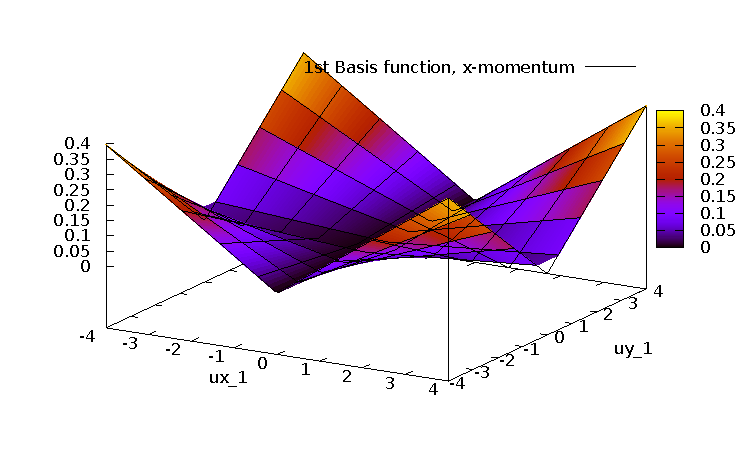
\includegraphics[scale=\zoomfactor]{{{standardwerte_nach_ux1_uy1_ord1/10.0_10.0_10.0_x_0.0_0.0_y_0.0_0.0f0}}}
  }
  \subfigure[] {
    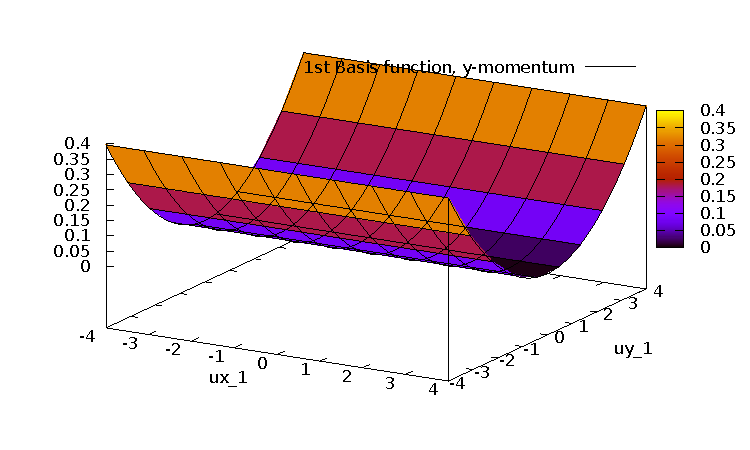
\includegraphics[scale=\zoomfactor]{{{standardwerte_nach_ux1_uy1_ord1/10.0_10.0_10.0_x_0.0_0.0_y_0.0_0.0f1}}}
  }
  \subfigure[] {
    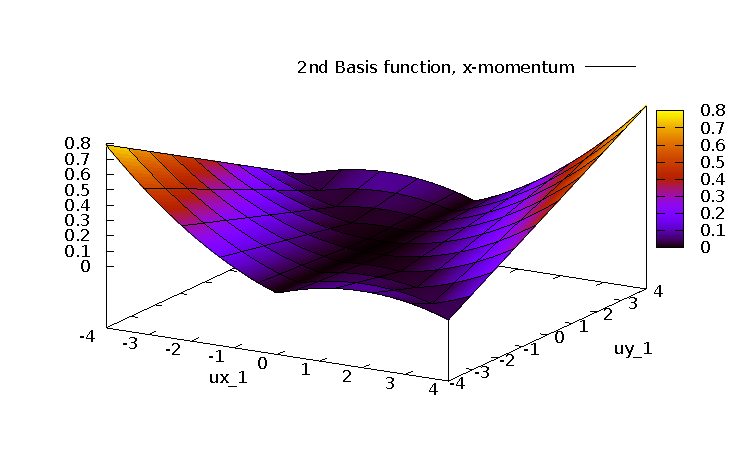
\includegraphics[scale=\zoomfactor]{{{standardwerte_nach_ux1_uy1_ord1/10.0_10.0_10.0_x_0.0_0.0_y_0.0_0.0f2}}}
  }
  \subfigure[] {
    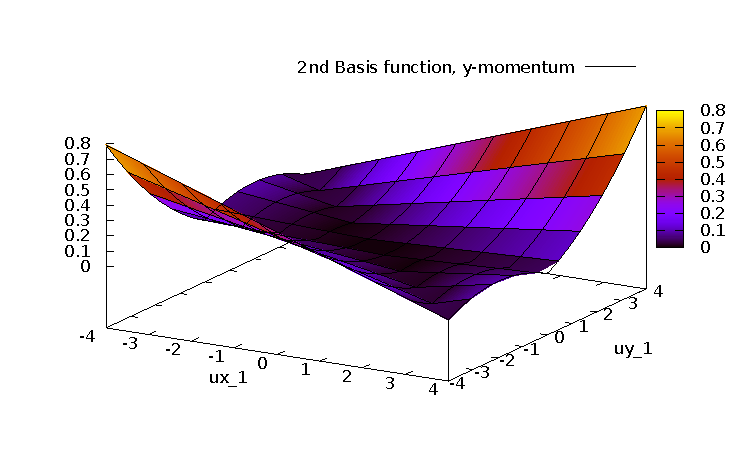
\includegraphics[scale=\zoomfactor]{{{standardwerte_nach_ux1_uy1_ord1/10.0_10.0_10.0_x_0.0_0.0_y_0.0_0.0f3}}}
  }
  \subfigure[] {
    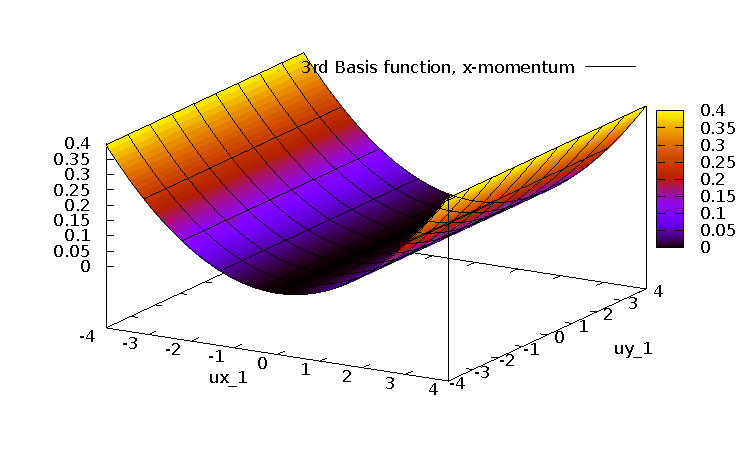
\includegraphics[scale=\zoomfactor]{{{standardwerte_nach_ux1_uy1_ord1/10.0_10.0_10.0_x_0.0_0.0_y_0.0_0.0f4}}}
  }
  \subfigure[] {
    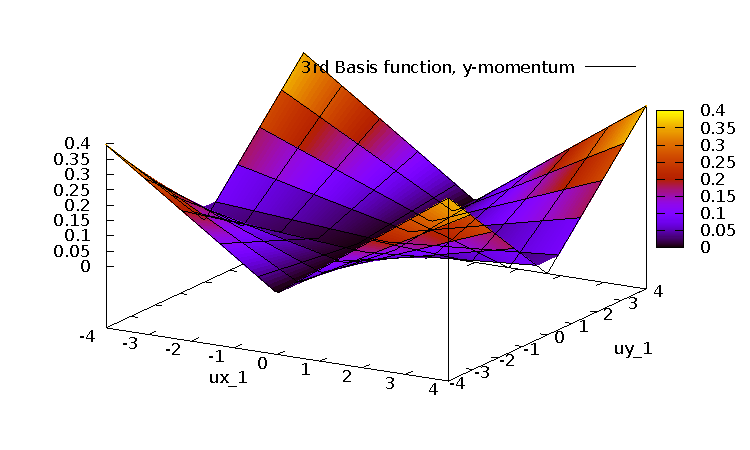
\includegraphics[scale=\zoomfactor]{{{standardwerte_nach_ux1_uy1_ord1/10.0_10.0_10.0_x_0.0_0.0_y_0.0_0.0f5}}}
  }
\caption{Basis functions of order 1. Variables $u_{x,1}$ and $u_{y,1}$ are the axes of the plots. All height values are set to 10, all remaining momentums set to 0.}
\label{fig:standardwerte_nach_ux1_ux2_ord1}
\end{figure}
